% Machine translated from the Danish original, ../danish/ad-problems-april-2026.tex
\noindent\emph{This problem set has been machine translated from the Danish original.}
\medskip

\section*{Multiple-choice}\label{sec:mc}

\placeholder{Where to enter the multiple-choice answers, e.g.\ the multiple-choice module of the exam system.}

\multiplechoicestart


\question{Asymptotic bounds}
Below are a number of running-time expressions. Which running time grows asymptotically slowest?
\oneanswer
\optionsstart
\answer{$n^2 + n \log n$}
\answer{$n^{\log_2(3)} + 1000\, n$}
\answer{$n \log n + \sqrt{n}$}
\answer{$2^n + n^{100}$}
\answer{$\log(4^n)$}\correct
\optionsend
\explanation{
We compare by simplifying each expression to its dominant term:
\[
n^2+n \log n=\Theta(n^2), \qquad
n^{\log_2 3}+1000\, n=\Theta(n^{\log_2 3}),
\]
\[
n \log n+\sqrt{n}=\Theta(n \log n), \qquad
2^n+n^{100}=\Theta(2^n).
\]
\[
\log(4^n)=n \log 4=\Theta(n).
\]
The slowest-growing (and hence fastest) one is $\Theta(n)$, that is, $\log(4^n)$.
}


\question{Recurrences}
Assume that $n$ is a power of $3$ and that $T(1)=1$. Consider the recurrence
\[
T(n) = 5\, T(n/3) + O(n \log n).
\]
What is the solution to the recurrence?
\oneanswer
\optionsstart
\answer $T(n) = \Theta(n^{\log_3(5)} \log n)$
\answer $T(n) = \Theta(n^{\log_3(5)})$\correct
\answer $T(n) = \Theta(n^{\log_5(3)} \log n)$
\answer $T(n) = \Theta(n^{\log_5(3)})$
\optionsend
\explanation{Write the recurrence in the form $T(n)=aT(n/b)+f(n)$ with $a=5$, $b=3$ and $f(n)=O(n \log n)$.
We have $n^{\log_b a}=n^{\log_3 5}$. Choose $\varepsilon < \log_3(5) - 1$; then
\(
n \log n = O\bigl(n^{\log_3(5)-\varepsilon}\bigr)
\).
Hence $f(n)=O(n^{\log_3 5-\varepsilon})$, and the master theorem (case 1) gives
\(
T(n)=\Theta(n^{\log_3 5}).
\)
The other options are therefore incorrect.}



\question{Divide and conquer}
A recursive algorithm {\sc SortAndRule} on an input of size $n$ (a power of~2) consists of three parts:
\begin{itemize}
    \item Sorting the input in time $\Theta(n \log n)$
    \item Four recursive calls on subproblems of size $n/2$
    \item A combine step that runs in time $\Theta(n)$
\end{itemize}
For input size $n=1$, {\sc SortAndRule} runs in time $T(1)=1$.
Which of the recurrences below best describes the running time $T(n)$ of {\sc SortAndRule}?
(You do not need to solve the recurrences, only determine which one corresponds directly to the algorithm.)
\oneanswer
\optionsstart
\answer $T(n) = T(n/4)/2 + \Theta(n)$
\answer $T(n) = 2\, T(n/2) + \Theta(n)$
\answer $T(n) = 4\, T(n/2) + \Theta(n)$
\answer $T(n) = T(n/4)/2 + \Theta(n \log n)$
\answer $T(n) = 2\, T(n/4) + \Theta(n \log n)$
\answer $T(n) = 4\, T(n/2) + \Theta(n \log n)$\correct
\optionsend
\explanation{The four recursive calls on subproblems of size $n/2$ are expressed by $4 T(n/2)$.
The combine step and the sorting step take total time $\Theta(n \log n)$, which is added.
}


\question{Loop invariants}
Consider the following algorithm, which takes as input an array $A[1\!:\!n]$ and a natural number $n$.
\begin{codebox}
\Procname{$\proc{MaximalMystery}(A,n)$}
\li $m \gets A[1]$
\li \For $i \gets 2$ \To $n$
\li \Do \If $A[i] > m$
\li \Then $m \gets A[i]$\End\End
\li \Return $m$
\end{codebox}
After each iteration of lines 3--4 we still regard the variable $i$ as unchanged; its value is changed only at the beginning of the next iteration.
Which of the following statements is a correct loop invariant of the \textbf{for} loop?
\multipleanswers
\optionsstart
\answer{At the start of each iteration, $m = \max\{A[1],\dots,A[i]\}$}
\answer{At the start of each iteration, $m = \max\{A[1],\dots,A[i-1]\}$}\correct
\answer{After each iteration, $m \geq \min \{A[1],\dots,A[i]\}$}\correct
\answer{After each iteration, $m \geq \min \{A[1],\dots,A[i-1]\}$}\correct
\answer{After each iteration, $m = A[i]$}
\answer{After each iteration, $m = A[i-1]$}
\optionsend
\explanation{We first argue that option 2 is correct. Before a given iteration, the algorithm has already processed the elements $A[1],\dots,A[i-1]$, so $m$ contains their maximum. During the iteration, $A[i]$ is compared with $m$, after which the invariant again holds for the next iteration. It follows that we always have $m\geq \min \{A[1],\dots,A[i-1]\} \geq \min \{A[1],\dots,A[i]\}$. The other invariants fail for $i=2$ if $A[1]=2$ and $A[2]=1$ (options 1 and 6) or if $A[1]=1$ and $A[2]=2$ (option 5).}



\question{Running-time analysis}
Let \proc{RB-Tree-Create}$()$ denote a procedure that creates a red-black search tree (with no keys) as described in CLRS Chapter 13.
The procedure \proc{RB-Tree-Search}$(x,k)$ searches for the key $k$ in a red-black search tree with root $x$ (returning $T.nil$ if the key is not present), the procedure \proc{RB-Insert}$(T,z)$ inserts a node $z$ into a red-black tree $T$, and the procedure \proc{RB-Node}$(k)$ creates a node containing the key $k$.

Consider the following algorithm, which determines whether two arrays $A[1\!:\!n]$ and $B[1\!:\!m]$, each containing a sequence of keys (not necessarily sorted), have an element in common.

\begin{codebox}
  \Procname{$\proc{HasCommonElement}(A,B,n,m)$}
  \li $T \gets \proc{RB-Tree-Create}()$
  \li \For $i \gets 1$ \To $n$ \Do
  \li $\proc{RB-Insert}(T, \proc{RB-Node}(A[i]))$ \End
  \li \For $j \gets 1$ \To $m$ \Do
  \li \If {\bf not} $\proc{RB-Tree-Search}(T.root, B[j]) == T.nil$ \Do
  \li \Return \const{true}\End\End
  \li \Return \const{false}
\end{codebox}
What is the asymptotic worst-case running time of the algorithm over all input arrays of length~$n$ and $m$, respectively?
\oneanswer
\optionsstart
\answer{$\Theta(n \log n + m)$}
\answer{$\Theta(n \log m + m)$}
\answer{$\Theta(n \log n + m \log m)$}
\answer{$\Theta(n \log m + m \log m)$}
\answer{$\Theta(n \log n + m \log n)$}\correct
\answer{$\Theta(n \log m + m \log n)$}
\optionsend
\explanation{
The first loop inserts $n$ elements into the red-black tree. Insertion $i$ costs
$\Theta(\log i)$, so the total is $\sum_{i=1}^{n} \Theta(\log i) = \Theta(n \log n)$.
The second loop performs up to $m$ searches in a tree with $n$ keys, so each search costs
$\Theta(\log n)$, and the total is $\Theta(m \log n)$ in the worst case (if there is no common element).
Altogether this gives $\Theta(n \log n + m \log n)$.
}



\question{Amortized analysis}
Consider dynamic tables as described in CLRS Section 16.4.1 (without deletions), but with the following variant of \proc{Table-Insert}$(T,x)$, in which the table size is expanded by a factor~$k$, where $k\geq 2$ is an integer parameter:

\begin{codebox}
  \Procname{$\proc{Table-Insert}_k(T,x)$}
  \li \If $T.size$ == $0$ \Do
  \li allocate $T.table$ with $1$ slot
  \li $T.size \gets 1$ \End
  \li \If $T.num == T.size$ \Do
  \li allocate $\mathit{new\text{-}table}$ with $k \cdot T.size$ slots
  \li insert all items in $T.table$ into $\mathit{new\text{-}table}$
  \li free $T.table$
  \li $T.table \gets \mathit{new\text{-}table}$
  \li $T.size \gets k \cdot T.size$ \End
  \li insert $x$ into $T.table$
  \li $T.num \gets T.num + 1$
\end{codebox}

Assume that a new table can be allocated in constant time, regardless of its length.
CLRS Section 16.4.1 uses the potential function $\Phi(T) = 2(T.num - T.size/2)$ for the analysis. Which of the potential functions below is best suited for an amortized analysis of \proc{Table-Insert}$_k$ showing that the time per insertion is $O(1)$, independently of $k$?
\oneanswer
\optionsstart
\answer $\Phi(T) = 2\,(T.num - T.size/2)$
\answer $\Phi(T) = 2\,(T.num - T.size/k)$\correct
\answer $\Phi(T) = k\,(T.num - T.size/2)$
\answer $\Phi(T) = k\,(T.num - T.size/k)$
\optionsend
\explanation{
Expressions with the factor $(T.num - T.size/2)$ can become negative for $k>2$ and therefore do not give valid potential functions.
The expression $k(T.num - T.size/k)$ increases by $k$ each time $T.num$ is incremented by 1, so it leads to an upper bound of $O(k)$ on the amortized cost.
The remaining option is $\Phi(T) = 2(T.num - T.size/k)$, which works:
On an expansion, $\Theta(T.size)$ elements are copied, so the potential must drop by a corresponding amount exactly when $T.num = T.size$.
With $\Phi(T)=2(T.num - T.size/k)$ the potential increases by a constant on an ordinary insertion (since $T.num$ is incremented by 1), which gives constant amortized cost in the cheap cases.
When the table is expanded, $T.size$ changes from $s$ to $ks$, while $T.num=s$. Hence $\Phi(T') = 2(s - ks/k) = 0$, so the potential drops sharply and pays for the copying.
}




\question{LSM trees}
Consider a simple LSM tree, as described in the note on LSM trees, in which all sorted lists have a length that is a power of $2$, and in which for each size $2^i$ there is at most one (sorted) list. What can be said about the number of binary searches (in nonempty lists) that must be performed to search for a key in an LSM tree with $n > 15$ elements?
\multipleanswers
\optionsstart
\answer{Never greater than $\lg\lg(n+1)$}
\answer{Never greater than $\lg(n+1)$}\correct
\answer{Never less than $\lg\lg(n+1)$}
\answer{Never less than $\lg(n+1)$}
\optionsend
\explanation{There can be at most one nonempty list of each size $2^i$, so the number of nonempty lists is at most the number of bits in $n$, i.e., $\lfloor \log_2 n \rfloor+1 \leq \lg(n+1)$, and this bound is tight. If $n$ is a power of 2, only one list needs to be searched.}



\question{Binary search trees}
Consider an empty binary search tree (BST) without balancing, as described in CLRS Chapter~12.
We insert keys in this order:
\begin{center}
7,\,3,\,10,\,1,\,5,\,8,\,12,\,4
\end{center}
What is the result of \proc{Inorder-Tree-Walk}$(r)$, i.e.,~an \emph{inorder} traversal of the tree starting at the root $r$, after all insertions?
\oneanswer
\optionsstart
\answer{The result is $1,3,4,5,7,8,10,12$}\correct
\answer{The result is $1,3,4,5,8,7,10,12$}
\answer{The result is $1,3,5,4,7,8,10,12$}
\answer{The result is $1,3,5,4,8,7,10,12$}
\optionsend
\explanation{In a binary search tree, an inorder traversal always yields the keys in sorted order. The inserted keys are $1,3,4,5,7,8,10,12$ in increasing order, so the inorder result is exactly this sequence.}



\question{Red-black search trees}
Consider this red-black binary search tree, where the leaves are omitted from the drawing:
%
\begin{center}
\begin{tikzpicture}[-,>=stealth,level/.style={sibling distance = 5cm/#1,
    level distance = 1cm}]
  \node [black] {41}
      child{ node [black] {12}
              child{ node [red] {3}
              }
              child{ node [red] {25}
              }
      }
      child{ node [red] {76}
              child{ node [black] {58}
              }
              child{ node [black] {94}
              }
          }
  ;
  \end{tikzpicture}
\end{center}

\medskip

Suppose we use the insertion algorithm {\sc RB-Insert} from CLRS Chapter 13 to insert the key~42. What happens to the tree?
\oneanswer
\optionsstart
\answer 42 is inserted as the right child of node 25 and colored red
\answer 42 is inserted as the right child of node 25 and colored black
\answer 42 is inserted as the left child of node 58 and colored red \correct
\answer 42 is inserted as the left child of node 58 and colored black
\optionsend
\explanation{
The position for the key is as the left child of node 58, since 42 is greater than the root node 41.
The new node is first inserted with color red.
Then {\sc RB-Insert-Fixup} is called, but no changes are made, since the parent (58) is black, so no red--red conflict arises.
}


\question{Bellman-Ford}
Consider the following directed, weighted graph $G$:
\begin{center}
\begin{tikzpicture}[>=Stealth,thick,node distance=2.4cm]
\node[circle,draw,minimum size=18pt] (s) {$s$};
\node[circle,draw,minimum size=18pt,right of=s] (a) {$a$};
\node[circle,draw,minimum size=18pt,below of=s] (b) {$b$};
\node[circle,draw,minimum size=18pt,right of=b] (c) {$c$};
\draw[->] (s) -- node[above] {$4$} (a);
\draw[->] (s) -- node[left] {$5$} (b);
\draw[->] (a) -- node[right] {$-2$} (b);
\draw[->] (a) -- node[right] {$6$} (c);
\draw[->] (b) -- node[below] {$1$} (c);
\end{tikzpicture}
\end{center}
We run $\proc{Bellman\text{-}Ford}(G,w,s)$ as described in CLRS Section 22.1, and in each iteration we go through the edges in the order $(s,a),(s,b),(a,b),(a,c),(b,c)$. What are the distances $(d[s],d[a],d[b],d[c])$ after the \emph{second} full iteration of the main loop (lines 2--4 in the CLRS pseudocode)?
\oneanswer
\optionsstart
\answer{$(d[s],d[a],d[b],d[c]) = (0,4,2,3)$}\correct
\answer{$(d[s],d[a],d[b],d[c]) = (0,4,2,6)$}
\answer{$(d[s],d[a],d[b],d[c]) = (0,4,3,3)$}
\answer{$(d[s],d[a],d[b],d[c]) = (0,4,3,6)$}
\answer{$(d[s],d[a],d[b],d[c]) = (0,4,5,3)$}
\answer{$(d[s],d[a],d[b],d[c]) = (0,4,5,6)$}
\optionsend
\explanation{Initialization: $d[s]=0$ and the others are $\infty$. First iteration: relaxing $(s,a)$ gives $d[a]=4$, relaxing $(s,b)$ gives $d[b]=5$, relaxing $(a,b)$ gives $d[b]=2$, relaxing $(a,c)$ gives $d[c]=10$, relaxing $(b,c)$ gives $d[c]=3$, so after the first iteration we have $(0,4,2,3)$. In the second iteration none of the edges can improve these values, so the distances remain $(0,4,2,3)$.}


\newpage

\question{Complete the algorithm}
Consider the following algorithm (with an unspecified part), which takes as input an array of integers $A[1\!:\!n]$ and positive integers $n$, $k$.
The algorithm must return the largest sum that can be obtained by choosing at most $k$ elements from $A[1\!:\!n]$ (an empty sum, with sum $0$, is allowed), i.e.,~we must find $\max_{|I|\leq k}\sum_{\ell\in I} A[\ell]$.
The algorithm works by computing an array $B[0\!:\!n, 0\!:\!k]$, where $B[i,j]$ is the largest sum $\sum_{\ell\in I} A[\ell]$ that can be obtained by choosing $I\subseteq \{1,\dots,i\}$ with $|I|=j$ elements, or $-\infty$ if no such set exists.
\begin{codebox}
\Procname{$\proc{TopKSum}(A,n,k)$}
\li let $B[0\!:\!n, 0\!:\!k]$ be a new table
\li \For $i \gets 0$ \To $n$\Do
\li $B[i,0] \gets 0$\End
\li \For $j \gets 1$ \To $k$
\li \Do $B[0,j] \gets -\infty$\End
\li \For $i \gets 1$ \To $n$
\li \Do \For $j \gets 1$ \To $k$
\li \Do $B[i,j] \gets$ INSERT CODE HERE\End\End
\li \Return $\max \{B[n,i] \; | \; i=0,\dots,k\}$
\end{codebox}
Which expression should replace ``INSERT CODE HERE'' to obtain a correct algorithm?
\oneanswer
\optionsstart
\answer{$B[i-1,j-1] + A[i]$}
\answer{$\max\{B[i-1,j],B[i-1,j]+A[i]\}$}
\answer{$B[i-1,j] + A[i]$}
\answer{$\max\{B[i-1,j],B[i-1,j-1]+A[i]\}$}\correct
\answer{$B[i-1,j] + A[i-1]$}
\answer{$\max\{0,B[i-1,j-1]+A[i]\}$}
\optionsend
\explanation{When we see $A[i]$, the best sum with exactly $j$ chosen elements in the prefix $A[1\!:\!i]$ can either (1) not choose $A[i]$, which gives the old value $B[i-1,j]$, or (2) choose $A[i]$, which requires that we had previously chosen exactly $j-1$ elements in $A[1\!:\!i-1]$, and gives $B[i-1,j-1]+A[i]$. Therefore the update is $B[i,j]\gets\max\{B[i-1,j],B[i-1,j-1]+A[i]\}$.}




\question{Minimum spanning tree}
Consider the minimum spanning tree problem on this graph, with an unspecified weight $x$:
\begin{center}
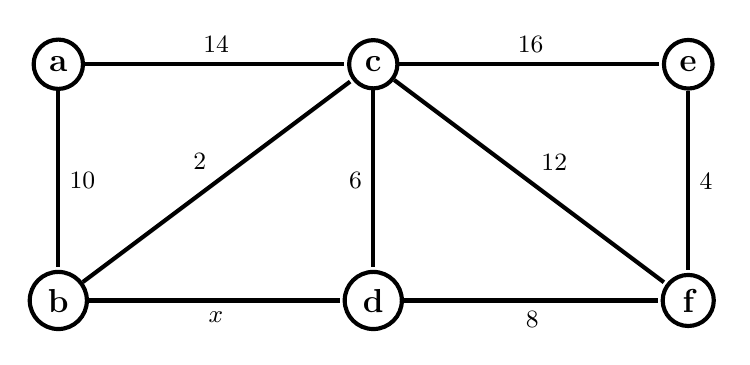
\begin{tikzpicture}[-,>=stealth,shorten >=1pt,auto,
  main node/.style={circle,draw,font=\large\bfseries}, line width=1.5pt]
\node[main node] (a) at (1,1.5) {a};
\node[main node] (b) at (1,-1.5) {b};
\node[main node] (c) at (5,1.5) {c};
\node[main node] (d) at (5,-1.5) {d};
\node[main node] (e) at (9,1.5) {e};
\node[main node] (f) at (9,-1.5) {f};

\path[every node/.style={font=\small}]
(a) edge node {10} (b)
(a) edge node {14} (c)
(b) edge node {2} (c)
(b) edge[below] node {$x$} (d)
(c) edge[left] node {6} (d)
(c) edge[above] node {16} (e)
(d) edge[below] node {8} (f)
(e) edge node {4} (f)
(c) edge node {12} (f);
\end{tikzpicture}
\end{center}

For which values of $x$ is the edge \{{\bf b},{\bf d}\} in the minimum spanning tree?
\multipleanswers
\optionsstart
\answer $x=1$ \correct
\answer $x=3$ \correct
\answer $x=5$ \correct
\answer $x=7$
\answer $x=9$
\answer $x=11$
\answer $x=13$
\optionsend

\explanation{
One can run Kruskal's algorithm for each choice of $x$. Alternatively, one can observe that Prim's algorithm with start vertex $d$ includes the edge \{{\bf b},{\bf d}\} if $x<6$. If $x>6$, the edges \{{\bf c},{\bf d}\} and \{{\bf b},{\bf c}\} are included instead, i.e., \{{\bf b},{\bf d}\} is not included.
}



\question{Disjoint sets}
We consider tree representations of disjoint sets, as described in CLRS Section 19.3, using the \emph{weighted-union} heuristic without path compression.
Assume that $n$ and $m$ are large integers (not bounded by any constant) with $m < n - 1$.
An algorithm makes $n$ calls to {\sc Make-Set} and $m$ calls to {\sc Union}.
What holds for the running time of a call to {\sc Find-Set}$(x)$?
\multipleanswers
\optionsstart
\answer The time is $\Omega(\log n)$ for all $x$
\answer The time is $O(\log n)$ for all $x$\correct
\answer The time is $\Omega(\log m)$ for all $x$
\answer The time is $O(\log m)$ for all $x$\correct
\optionsend
\explanation{ The height of a tree with $k$ nodes is at most $\log k$ because of the weighted-union heuristic. If we perform $m$ {\sc Union} operations, there can be at most $m+1$ elements in each tree, i.e.,~the time is $O(\log m)$, which is also $O(\log n)$ since $m<n$.
If $x$ is in a component of size 1 (there is at least one such component), then the time for {\sc Find-Set}$(x)$ is constant, i.e.,~not $\Omega(\log n)$ or $\Omega(\log m)$.
}



\question{Shortest paths}
Consider the following weighted graph $G=(V,E)$:
\begin{center}
  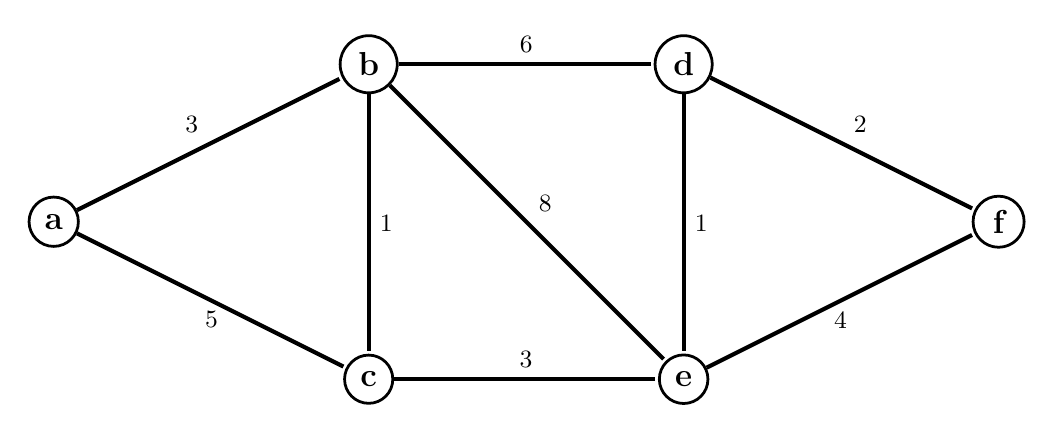
\begin{tikzpicture}[-,>=stealth,shorten >=1pt,auto,
      main node/.style={circle,draw,font=\large\bfseries,line width=1pt}, line width=1.5pt]
  \node[main node] (a) at (0,0) {a};
  \node[main node] (b) at (4,2) {b};
  \node[main node] (c) at (4,-2) {c};
  \node[main node] (d) at (8,2) {d};
  \node[main node] (e) at (8,-2) {e};
  \node[main node] (f) at (12,0) {f};
  \path[every node/.style={font=\small}]
  (a) edge node {3} (b)
  (a) edge[below] node {5} (c)
  (b) edge node {1} (c)
  (b) edge node {6} (d)
  (b) edge node {8} (e)
  (c) edge node {3} (e)
  (d) edge node {1} (e)
  (d) edge node {2} (f)
  (e) edge[below] node {4} (f);
  \end{tikzpicture}
\end{center}

How many edges are there on the shortest path from vertex {\bf a} to vertex~{\bf f}?
\oneanswer
\optionsstart
\answer 3 edges
\answer 4 edges
\answer 5 edges \correct
\answer 10 edges
\answer 11 edges
\answer 12 edges
\optionsend

\explanation{
The graph is undirected, i.e.,~in an adjacency-list representation there are two edges between each pair of connected vertices.
Run Dijkstra's algorithm on the adjacency-list representation with start vertex A.
This gives the shortest path A--B--C--E--D--F, which has 5 edges.
(The length, i.e., the total weight of the shortest path, is 10.)
}



\question{Choice of algorithm}
We want to find a path through a 2-dimensional grid from a start position $S$ to an end position $T$ that has as low a cost as possible.

\begin{center}
\begin{tikzpicture}[scale=0.5, line cap=round, line join=round]
  % Grid size: 16 columns (x=0..16), 8 rows (y=0..8)
  % Coordinate system: (0,8) is top-left corner; (16,0) is bottom-right corner.

  % Light grid (optional)
  \draw[gray!25, very thin] (0,0) grid (10,6);

  % Mark start and goal cells
  \node[draw, circle, inner sep=1.5pt] at (0.5,5.5) {\scriptsize S};
  \node[draw, circle, inner sep=1.5pt] at (9.5,0.5) {\scriptsize T};

  \node at (2.5,5.5) {\scriptsize -2};
  \node at (4.5,4.5) {\scriptsize -1};
  \node at (1.5,2.5) {\scriptsize -2};
  \node at (3.5,1.5) {\scriptsize -2};
  \node at (8.5,3.5) {\scriptsize -1};
  \node at (7.5,0.5) {\scriptsize -1};
  \begin{scope}[on background layer]
 \draw[cyan]
    (0.5,5.5) -- (2.5,5.5) -- (2.5,4.5) -- (7.5,4.5) -- (7.5,3.5) -- (9.5,3.5)
    -- (9.5,0.5);
    \end{scope}
\end{tikzpicture}
\end{center}

In each step one can move one position horizontally or vertically, which has a cost of~1.
Some cells contain a negative number: moving to such a cell reduces the cost by the magnitude of the number.
The path shown has a cost of 10: there are 14 steps, from which 2, 1 and 1 are subtracted.
The cheapest path has a cost of 9.
Which of the algorithms below is best suited to be part of an algorithm that solves this problem?
\oneanswer
\optionsstart
\answer The Bellman-Ford algorithm \correct
\answer Dijkstra's algorithm
\answer The longest common subsequence algorithm
\answer Prim's algorithm
\answer The rod-cutting algorithm
\optionsend
\explanation{The problem can be expressed as a shortest-path problem on a graph defined from the grid. The negative contributions can be modeled as an edge internal to each cell. Since there are negative edge weights, we cannot use Dijkstra's algorithm but must use the slower Bellman-Ford algorithm.
}




\question{Closest pair of points}
CLRS online Chapter 33, Section 4, presents a divide-and-conquer algorithm with running time $O(n \log n)$ for finding the closest pair of points in a set of 2-dimensional points.
The algorithm starts by sorting the points by $y$-coordinate in time $O(n \log n)$ and then solves the problem with a recursive algorithm.
Now assume that the input to the algorithm is already sorted, so that the sorting step is not needed.
What holds for the running time of the recursive part of the algorithm, i.e., without the sorting step?
\oneanswer
\optionsstart
\answer For all inputs the algorithm runs in time $\Theta(\log n)$
\answer For all inputs the algorithm runs in time $\Theta(n)$
\answer For all inputs the algorithm runs in time $\Theta(n \log n)$ \correct
\answer For all inputs the algorithm runs in time $\Theta(n^2)$
\optionsend
\explanation{ The recurrence that determines the running time of the recursive algorithm is still $T(n) = 2 T(n/2) + \Theta(n)$, which has the solution $T(n) = \Theta(n \log n)$.
}



\question{Longest common subsequence}
What is the length of a longest common subsequence of the strings {\tt AABBCDAAB} and {\tt ABDAACBB}?
\oneanswer
\optionsstart
\answer Length 1
\answer Length 2
\answer Length 3
\answer Length 4
\answer Length 5
\answer Length 6\correct
\answer Length 7
\optionsend
\explanation{Run the LCS algorithm from CLRS:

\begin{center}
\begin{tabular}{c|c|c|c|c|c|c|c|c|c||}
    &   & A & B & D & A & A & C & B & B\\
    \hline
     & 0 & 0 & 0 & 0 & 0 & 0 & 0 & 0 & 0\\
     \hline
    A & 0 & $\nwarrow1$ & $\leftarrow1$ & $\leftarrow1$ & $\nwarrow1$ & $\nwarrow1$ & $\leftarrow1$ & $\leftarrow1$ & $\leftarrow1$ \\
    A & 0 & $\nwarrow1$ & $\uparrow1$ & $\uparrow1$ & $\nwarrow2$ & $\nwarrow2$ & $\leftarrow2$ & $\leftarrow2$ & $\leftarrow2$ \\
    B & 0 & $\uparrow1$ & $\nwarrow2$ & $\leftarrow2$ & $\uparrow2$ & $\uparrow2$ & $\uparrow2$ & $\nwarrow3$ & $\nwarrow3$ \\
    B & 0 & $\uparrow1$ & $\nwarrow2$ & $\uparrow2$ & $\uparrow2$ & $\uparrow2$ & $\uparrow2$ & $\nwarrow3$ & $\nwarrow4$ \\
    C & 0 & $\uparrow1$ & $\uparrow2$ & $\uparrow2$ & $\uparrow2$ & $\uparrow2$ & $\nwarrow3$ & $\uparrow3$ & $\uparrow4$ \\
    D & 0 & $\uparrow1$ & $\uparrow2$ & $\nwarrow3$ & $\leftarrow3$ & $\leftarrow3$ & $\uparrow3$ & $\uparrow3$ & $\uparrow4$ \\
    A & 0 & $\nwarrow1$ & $\uparrow2$ & $\uparrow3$ & $\nwarrow4$ & $\nwarrow4$ & $\leftarrow4$ & $\leftarrow4$ & $\uparrow4$ \\
    A & 0 & $\nwarrow1$ & $\uparrow2$ & $\uparrow3$ & $\nwarrow4$ & $\nwarrow5$ & $\leftarrow5$ & $\leftarrow5$ & $\leftarrow5$ \\
    B & 0 & $\uparrow1$ & $\nwarrow2$ & $\uparrow3$ & $\uparrow4$ & $\uparrow5$ & $\uparrow5$ & $\nwarrow6$ & $\nwarrow6$ \\
    \hline
\end{tabular}
\end{center}

An LCS is {\tt ABDAAB}, which has length 6.
}




\question{Work and span}
Consider the following parallel algorithm, which finds the maximum in an array $A[1\!:\!n]$ by divide and conquer.

\begin{codebox}
\Procname{$\proc{Parallel-Max}(A, p, q)$}
\li \If $p == q$
\li \Then \Return $A[p]$
\li \Else
\li     $mid \gets \lfloor (p+q)/2 \rfloor$
\li     \Spawn $m_1 \gets \proc{Parallel-Max}(A, p, mid)$
\li     $m_2 \gets \proc{Parallel-Max}(A, mid+1, q)$
\li     \Sync
\li     \If $m_1 > m_2$
\li     \Then \Return $m_1$
\li     \Else \Return $m_2$\End
\end{codebox}

\noindent
Assume that $n = q-p+1$. What are the work and span of the algorithm?
\oneanswer
\optionsstart
\answer Work $T_1=\Theta(\log n)$, span $T_\infty=\Theta(\log n)$
\answer Work $T_1=\Theta(\log n)$, span $T_\infty=\Theta(n)$
\answer Work $T_1=\Theta(n)$, span $T_\infty=\Theta(\log n)$ \correct
\answer Work $T_1=\Theta(n)$, span $T_\infty=\Theta(n)$
\answer Work $T_1=\Theta(n \log n)$, span $T_\infty=\Theta(\log n)$
\answer Work $T_1=\Theta(n \log n)$, span $T_\infty=\Theta(n)$
\optionsend

\explanation{
Each recursive step splits the input into two halves and performs constant extra work.
The recurrence for the work is
$T_1(n)=2T_1(n/2)+O(1)=\Theta(n)$.
The span is determined by the longest chain of dependencies:
$T_\infty(n)=T_\infty(n/2)+O(1)=\Theta(\log n)$.
The algorithm thus has linear work and logarithmic span.
}




\multiplechoiceend

\newpage

\section*{Written problems}\label{sec:written}

% Machine translated from the Danish original, ../danish/skriftlige.tex
{\bf Written problems:} \placeholder{How the answers are submitted, e.g.\ the file format and exam system, and whether drawings made on a tablet may be inserted.}
\begin{itemize}
    \item Use \emph{one page for each subquestion, in the same order as in the problem set.}
    \item The number/letter of the subquestion (e.g.\ 19 or 20.a) must be stated.
\end{itemize}


\section{Huffman trees (4\%)}

We consider the algorithm for constructing Huffman codes in CLRS Section 15.3.

\subquestion{}{Draw the Huffman tree that the algorithm computes for the alphabet $C =\{A,E,I,O,U,Y\}$ with frequencies $f_A=4$, $f_E=1$, $f_I=3$, $f_O=7$, $f_U=6$, $f_Y=1$.
It is not necessary to put labels (0 and 1) on the edges, but give the frequencies in the leaves as well as in the internal nodes (see the example in CLRS Section~15.3).}

\explanation{The algorithm computes this tree (drawn without 0-1 labels on the edges):\medskip
\begin{center}
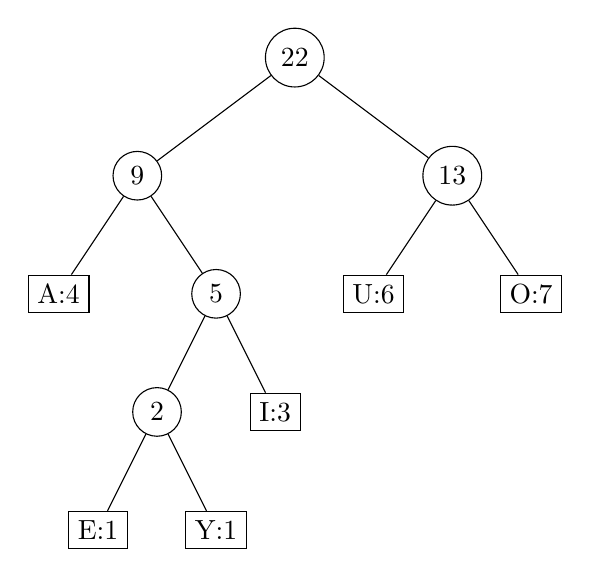
\begin{tikzpicture}[
  level distance=1.5cm,
  level 1/.style={sibling distance=4cm},
  level 2/.style={sibling distance=2cm},
  level 3/.style={sibling distance=1.5cm}
]
\node[circle,draw]{22}
  child {node[circle,draw]{9}
    child {node[rectangle,draw]{A:4}}
    child {node[circle,draw]{5}
      child {node[circle,draw]{2}
        child {node[rectangle,draw]{E:1}}
        child {node[rectangle,draw]{Y:1}}
      }
      child {node[rectangle,draw]{I:3}}
    }
  }
  child {node[circle,draw]{13}
    child {node[rectangle,draw]{U:6}}
    child {node[rectangle,draw]{O:7}}
  };
\end{tikzpicture}
\end{center}
}




\section{Largest common prefix sum (12\%)}

For an array $S[1\!:\!n]$, a \emph{prefix sum} of $S$ is defined as a number of the form $\sum_{i=1}^jS[i]$, for $j\in\{0,1,\ldots,n\}$.
In this problem we are given three arrays $A[1\!:\!n],B[1\!:\!n],C[1\!:\!n]$, all containing positive integers.
We want to find the largest number $x$ that is a prefix sum of each of $A$, $B$ and $C$.
In other words, it must be possible to write $x$ as $x=\sum_{i=1}^aA[i]=\sum_{i=1}^bB[i]=\sum_{i=1}^cC[i]$ for indices $a,b,c\in\{0,1,\ldots,n\}$.
Note that these indices $a,b,c$ are allowed to be different.

\subquestion{a)}
{Let $A=\langle 1,2,3,4\rangle$, $B=\langle 3,2,3,4\rangle$ and $C=\langle 1,1,1,4\rangle$.
What is the largest common prefix sum? Briefly justify your answer.}

\explanation{The answer is $3$, which can be written as the prefix sums $1+2=3=1+1+1$ in $A$, $B$ and $C$, respectively (we choose $a=2$, $b=1$, $c=3$). The only larger prefix sum of $C$ is~7, which is not a prefix sum of $A$ or $B$.}

\subquestion{b)}
{Describe an algorithm that finds the largest common prefix sum.
The input to the algorithm is the three arrays $A,B,C$ and their size $n$.
You may write pseudocode, but a clear and precise description in text is also sufficient.
To get full points, the running time must be $O(n)$.}

\explanation{
We can solve the problem with a greedy algorithm (but note that other solutions exist).
We define variables $x_A,x_B,x_C$, which are initially the sums of all numbers in $A,B,C$, respectively.
We also define indices $a=b=c=n$.
If $x_A$ is strictly greater than $x_B$ or $x_C$, we subtract $A[a]$ from $x_A$ and subtract $1$ from $a$, and similarly if $x_B$ or $x_C$ is greater than one of the others.
This corresponds to removing the last number from the prefix sum $x_A$.
When $x_A=x_B=x_C$, we return this value.
This happens after at most $3n$ iterations, at which point we will have $a=b=c=0$ and $x_A=x_B=x_C=0$.
Therefore the running time is $O(n)$.
In pseudocode it can be written as follows:

\begin{codebox}
\Procname{$\proc{LargestCommonPrefixSum}(A,B,C, n)$}
\li let $x_A=\sum_{i=1}^n A[i]$, $x_B=\sum_{i=1}^n B[i]$, $x_C=\sum_{i=1}^n C[i]$ and $a=b=c=n$
\li \While $x_A\neq x_B$ or $x_A\neq x_C$
\Do
\li     \If $x_A>x_B$ or $x_A>x_C$
\li     \Then $x_A=x_A-A[a]$
\li         $a=a-1$
\li     \ElseIf $x_B>x_A$ or $x_B>x_C$
     \li     \Then $x_B=x_B-B[b]$
\li         $b=b-1$
\li \Else
\li     $x_C=x_C-C[c]$
\li         $c=c-1$
\End
\End
\li \Return $x_A$
\end{codebox}
}


\subquestion{c)}
{Argue that the algorithm always finds the correct answer.}

\explanation{
We maintain the invariant that all three values $x_A,x_B,x_C$ are greater than or equal to the solution $x$.
Since all numbers in $A,B,C$ are positive, the invariant is true at the beginning.
If one of $x_A,x_B,x_C$, e.g.\ $x_A$, is greater than another, we can thus conclude from the invariant that $x_A$ is too large.
Hence the invariant holds again after we have removed the last number $A[a]$ from $x_A$.
}


\section{Algorithm analysis (12\%)} \label{sec:last}

Let $\proc{BinarySearch}(A, p, q, x)$ be the algorithm below, which implements binary search for~$x$ in an array $A[p\!:\!q]$ in time $O(\log n)$, where $p\leq q$ and $n = q-p+1$ is the number of elements, with $n>1$.
Assuming that $A[p\!:\!q]$ contains integers sorted in nondecreasing order, $\proc{BinarySearch}(A, p, q, x)$ returns {\sc true} if $x$ is in $A[p\!:\!q]$ and {\sc false} otherwise.

\begin{codebox}
\Procname{$\proc{BinarySearch}(A,p,q,x)$}
\li \While $p \le q$
\li \Do $mid \gets p + \lfloor (q-p)/2 \rfloor$
\li \If $A[mid] = x$
\li \Then \Return \const{true}
\li \Else \If $A[mid] < x$
\li \Then $p \gets mid + 1$
\li \Else $q \gets mid - 1$\End\End\End
\li \Return \const{false}
\end{codebox}

An array $A[1\!:\!n]$ is \emph{strictly bitonic} if there exists an index $i$ such that $A[1\!:\!i]$ is increasing and $A[i:n]$ is decreasing.
%
{\bf Example:} $A_1 = \langle 1, 2, 3, 5, 2, 1, 0\rangle$ is strictly bitonic because $A_1[1\!:\!4] = \langle 1, 2, 3, 5\rangle$ is increasing and $A_1[4:7] = \langle 5, 2, 1, 0\rangle$ is decreasing. $A_2 = \langle 1, 2, 3, 5, 2, 2, 0\rangle$ cannot be strictly bitonic because it has two consecutive identical values.

\subquestion{a)}{Give an example of a strictly bitonic array $A[1\!:\!n]$ and an element $x$ from $A$ for which $\proc{BinarySearch}(A, 1, n, x)$ returns \const{false} (even though $x$ is in $A$).}

\explanation{
For $A = \langle 3, 2, 1\rangle$ and $x=1$, $x$ is first compared with $2$ and then with $3$ in the next iteration.
\medskip
}

Let $\proc{ReverseBinarySearch}(A, p, q, x)$ have the same functionality as $\proc{BinarySearch}$, except that $A[p\!:\!q]$ is assumed to be sorted in \emph{reverse} order (nonincreasing order). We now consider the following recursive algorithm:
%
\begin{codebox}
\Procname{$\proc{BTS2}(A,p,q,x)$}
\li $mid \gets \lfloor (p+q)/2 \rfloor$
\li \If $A[mid]==x$
\li \Then \Return \const{true}
\End
\li \If $p \ge q$
\li \Then \Return \const{false}
\End
\li \If $A[mid] < A[mid+1]$
\Then
\li     \If \proc{BinarySearch}$(A,p,mid,x)$
\li     \Then \Return \const{true}
    \End
\li     \If \proc{BTS2}$(A,mid+1,q,x)$
\li     \Then \Return \const{true}
    \End
\li \Else
\li     \If \proc{ReverseBinarySearch}$(A,mid+1,q,x)$
\li     \Then \Return \const{true}
    \End
\li     \If \proc{BTS2}$(A,p,mid,x)$
\li     \Then \Return \const{true}
    \End
\End
\li \Return \const{false}
\end{codebox}
\subquestion{b)}{Write down a recurrence for the worst-case running time $T(n)$ of $\proc{BTS2}$ on an input of length $n$, and use it to derive an asymptotic upper bound on the running time. The analysis should be as precise as possible.}

\explanation{
In the worst case, $x$ is not in $A[p\!:\!q]$, i.e.,~the algorithm returns only after both the binary search and the recursive call have been made.
In this case the algorithm does constant work, one binary search on at most $n/2$
elements (time $O(\log n)$), and one recursive call on at most $n/2$
elements.
This gives the recurrence \(T(n)=T(n/2)+O(\log n)\).
It can be solved with the master method or with the substitution method, with the result
\(
T(n)=\Theta((\log n)^2)
\).
}

\subquestion{c)}{Assume that $A[1\!:\!n]$ is strictly bitonic. Argue that $\proc{BTS2}(A, 1, n, x)$ returns {\sc true} if $x$ is in $A[1\!:\!n]$ and {\sc false} otherwise.}

\explanation{
Let $A[1\!:\!n]$ be strictly bitonic with peak $i$, i.e.,~$A[1\!:\!i]$ is increasing and $A[i:n]$ is decreasing.
For a given interval $A[p\!:\!q]$, the test
$A[mid] < A[mid+1]$ determines whether $mid$ lies in the increasing
or the decreasing part.
If $A[mid] < A[mid+1]$, then $A[p\!:\!mid]$ is increasing,
and it is correct to use $\proc{BinarySearch}$ to determine whether $x$ is in $A[p\!:\!mid]$.
Otherwise $A[mid+1\!:\!q]$ is decreasing,
and it is correct to use $\proc{ReverseBinarySearch}$ to determine whether $x$ is in $A[mid+1\!:\!q]$.
If $x$ is not in the monotone half,
it can only be in the other half,
which is handled recursively.
The interval is halved in each step,
so by induction on the size of the interval
the algorithm returns {\sc true}
if and only if $x$ is in $A[1\!:\!n]$.
(The base case $p=q$ is handled by lines 2--5.)
}

\label{page:last}
